\section{Textual Entailment and Paraphrasing}
\begin{itemize}
	\item Textual entailment is defined as a directional relationship of text $T$ to hypothesis $H$
	\item We say $T$ entails $H$ if the meaning of $H$ can be inferred from the meaning of $T$
	\item Task of recognizing textual entailment aims for classifying a pair of sentences as whether they are an entailment or not (binary classifier). Can be used in different settings:
	\begin{itemize}
		\item \textit{Question-Answering}: A question answering system generates $n$ candidate solutions. The textual entailment recognizer must now decide which candidate solution is correct
		\item \textit{Summarization}: A summarization system sequentially generates new sentences to add to the summary in progress. The textual entailment recognizer should now identify whether a new sentence contains information that is already in the summary or not (redundancy checker).
	\end{itemize}
\end{itemize}
\subsection{Levels of Representation}
\begin{itemize}
	\item Determining the equivalence of the meaning of $T$ and $H$
	\item The representation of the $T$-$H$ pair is used to train a supervised model
	\item There are different levels of representation that can be used (all having their own benefits and drawbacks)
	\item \textbf{Lexical level}
	\begin{itemize}
		\item Solely looking on the words used in $T$ and $H$ (basically BoW of both sentences)
		\item Comparing the used words for similarity (are words of $H$ in $T$)
		\item Problem: structure of $H$ and $T$ cannot be fully captured by BoW
	\end{itemize}
	\item \textbf{Structural level}
	\begin{itemize}
		\item Build up syntactic structure (like parse tree from context-free grammar or dependency graph) for $T$ and $H$
		\item If $T$ contains same structures as $H$ (i.e. certain dependency edges, subtrees, ...), we predict the texts to be entailed
		\item However, it is hard to distinguish which edges should contribute to similarity and which not 
	\end{itemize}
	\item \textbf{Semantic level}
	\begin{itemize}
		\item The idea is to label words/phrases with semantic role in sentence
		\item Words are group into \textit{arguments} (such as person or place) and connected to \textit{predicates} (mostly verbs)
		\item Now we check whether semantic connections of $H$ are in $T$ or not
		\begin{figure}[ht]
			\centering
			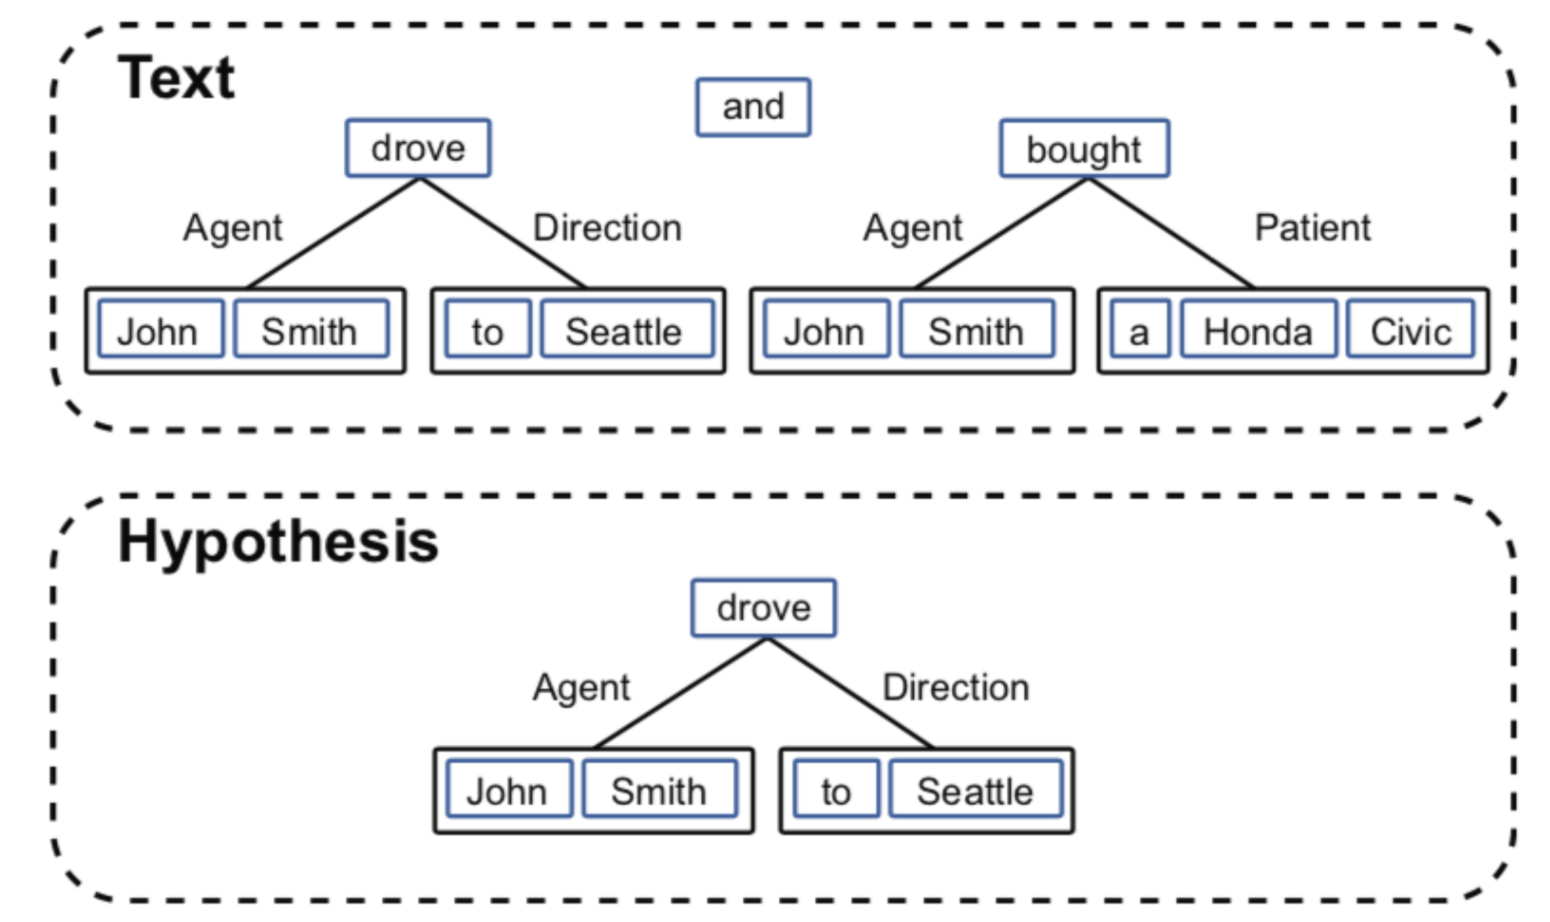
\includegraphics[width=0.4\textwidth]{figures/text_entailment_semantic_level.png}
		\end{figure}
	\end{itemize}
	\item \textbf{Knowledge Acquisition for RTE}
	\begin{itemize}
		\item To answer some text entailments, background/world knowledge is required (which words are synonyms, what is connected to a certain noun as i.e. a person/place...)
		\item Knowledge is mostly constrained to lexical-semantic between two words (synonym, hypnonymy, ...)
		\item But we can also model more complex relations like $X$ causes $Y$ $\implies$ $Y$ is a \textit{symptom} of $X$
		\item Such connections/knowledge can be retrieved from WordNet, Wikipedia, ...
		\item This leads to the \textbf{Extended Distributional Hypothesis}: if two paths occur in similar contexts, the meaning of the paths tend to be similar ($X$ \textit{solves} $Y$ compared to $X$ \textit{is a solution of }$Y$)
	\end{itemize}
\end{itemize}
\subsection{Recognizing Text Entailment Methods}
\begin{itemize}
	\item RTE depend on the representation which is used for $T$ and $H$
	\item Different approaches to model the classifier
	\item \textbf{Similarity-based approach}
	\begin{itemize}
		\item Pair with strong similarity score gets high entailment relation
		\item Similarity is measured by for example WordNet (how many edges to traverse to get to other word) and string similarity (length or even single letters)
	\end{itemize}
	\item \textbf{Alignment-based approaches}
	\begin{itemize}
		\item Use heuristics to align junk of words from $T$ to $H$
		\item For example, match phrase "\textit{purchase of $X$ to $Y$}" with "\textit{$Y$ acquired $X$}"
		\item However, we need a knowledge base to infer these relations
		\begin{figure}[ht]
			\centering
			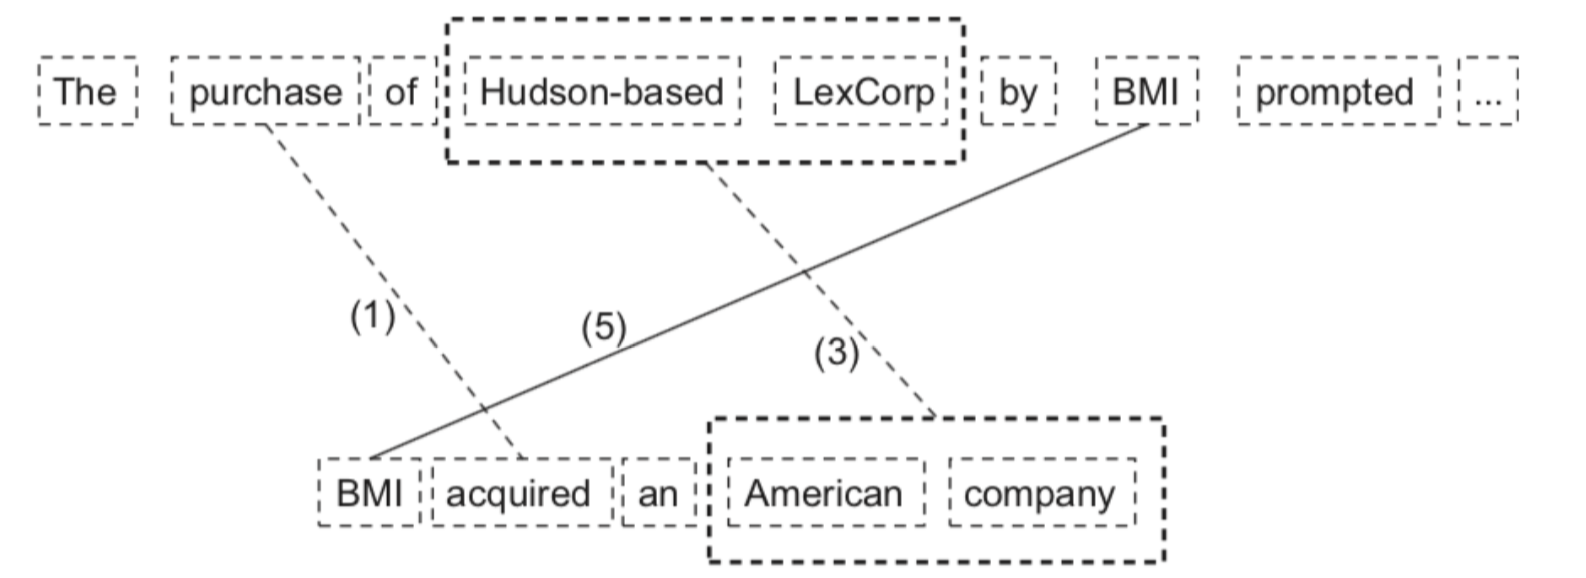
\includegraphics[width=0.4\textwidth]{figures/text_entailment_alginment_based_methods.png}
		\end{figure}
	\end{itemize}
	\item \textbf{Formal Logic approaches}
	\begin{itemize}
		\item Finding proof by theorem prover that $H$ can be proofed by $T$ 
		\item Convert statements in $T$ and $H$ into formal logic
		\item Problem: mostly the lack of background knowledge is the bottleneck, as the simplest mistakes/missing statements can stop this approach to get the correct result
	\end{itemize}
	\item \textbf{Edit distance-based approaches}
	\begin{itemize}
		\item Sequence of transformations that need to be applied on $T$ to get to $H$
		\item If the number of transformations is higher than specified threshold, classify relation as \texttt{false}
		\item Alternative for \textit{expensive} theorem prover
	\end{itemize}
	\item Evaluation done on dataset with 1,600 $T$-$H$ pairs with accuracy as metric. Lexical baseline is at about 58\%
\end{itemize}
\subsection{Current methods}
\begin{itemize}
	\item RTE datasets are mostly very small which limits the application of complex systems
	\item However, there are large Natural Language Inference datasets, where also neural networks can be trained on (different domains, for example image to text)
	\item We need datasets over multiple domains as otherwise the algorithms generalize poorly
	\item \textbf{Neural networks}
	\begin{itemize}
		\item Specifying features by hand for the input
		\item Using both hypothesis and text as input. Mostly, we classify then into classes \textit{entailment}, \textit{contradiction} and \textit{neutral} (not enough info to decide)
		\item Using various LSTM models with attention modules 
		\item Generative models create a hypothesis given the text and the class for which the hypothesis should be generated
		\item However, networks show to overfit on noise in the data (contradiction mostly contains negative words, entailments biased on animals and so on)
	\end{itemize}
\end{itemize}